% !TeX program = lualatex
% !BIB program = biber
% Lualatex is important to render TTF fonts; with pdflatex it's just the regular one
% ratio 16:9 -- https://tex.stackexchange.com/questions/14336/

% compile two versions, inspired by https://tex.stackexchange.com/a/1501
% use the script "compile-pdf.sh"
\newif\ifhandout
% if flags.tex does not exist, create an empty file to be able to compile in TeXstudio
\input{flags}

\ifhandout
\documentclass[12pt,aspectratio=169,handout]{beamer}
\else
\documentclass[12pt,aspectratio=169]{beamer}
\fi



% TODO change "leftfootertext" to your liking
\newcommand{\leftfootertext}{\insertsubtitle}  % just the \title{} text by default
%\newcommand{\leftfootertext}{RNNs and encoder-decoder architectures}  % Your name, for instance


% ------- RUB specifics ----------
% adjust for 16:9
% https://tex.stackexchange.com/questions/354022/modifying-the-margins-of-all-slides-in-beamer
\setbeamersize{text margin left=0.3cm,text margin right=4.5cm} 


% use Metropolis as the basis theme
\usetheme[subsectionpage=progressbar]{metropolis}
% blocks with background globally
\metroset{block=fill}


\usepackage{fontspec}
% RUB fonts need to be installed
% 'UprightFont = * Light' makes sure that the base font is RubFlama Light, which looks
% lighter than RubFlama Regular (would be too thick for slides)
\setsansfont[Scale=MatchLowercase, UprightFont = * Light, BoldFont = * Bold]{RubFlama}
%\setsansfont{Arial} % Open source alternative if you don't have RubFlama

% RUB color scheme
% Dark blue: 0; 53; 96; #003560
\definecolor{RUBDarkBlue}{RGB}{0, 53, 96}

% Light yellow (table fill, etc.); 238; 250; 196; #EEFAC4
\definecolor{RUBLightYellow}{RGB}{238, 250, 196}

%Light green: 141; 174; 16
\definecolor{RUBLightGreen}{RGB}{141, 174, 16}


\setbeamercolor{titlelike}{fg=RUBDarkBlue}
\setbeamercolor{subtitle}{fg=RUBLightGreen}
\setbeamercolor{separation line}{fg=RUBLightGreen}
\setbeamercolor{frametitle}{bg=white, fg=RUBDarkBlue}

% horizontal line on title page and sections
\setbeamercolor{alerted text}{fg=RUBLightGreen}


% Adjust footer bottom (too large by default)
\setbeamertemplate{footline}{%
  \begin{beamercolorbox}[wd=\textwidth, sep=2ex]{footline}%
    \usebeamerfont{page number in head/foot}%
    \usebeamertemplate*{frame footer}
    \hfill%
    \usebeamertemplate*{frame numbering}
  \end{beamercolorbox}%
}


% Lab name, numbering, etc. in footer
\setbeamertemplate{frame numbering}{TrustHLT --- Prof.\ Dr.\ Ivan Habernal \hspace*{1ex} \includegraphics[width=7em]{img/rub-logo.pdf}\hspace*{1ex}}

\setbeamertemplate{frame footer}{\hspace*{1ex}\insertframenumber \hspace*{2ex} \leftfootertext}

% adjust the background to be completely white
\setbeamercolor{background canvas}{bg=white}

% logos on the title page
\titlegraphic{%
	\begin{picture}(0,0)
		\put(435,0){\makebox(0,0)[rt]{\includegraphics[width=7em]{img/rub-logo.pdf}}}
		\put(435,-170){\makebox(0,0)[rt]{\includegraphics[width=4em]{img/logo-trusthlt.pdf}}}
		\put(435,-196){\makebox(0,0)[rt]{\includegraphics[width=9em]{img/logo-rctrust.pdf}}}
	\end{picture}%
}


% show TOC at every section start
\AtBeginSection{
	\frame{
		\vspace{2em}
		\sectionpage
		\hspace*{2.2em}\begin{minipage}{10cm}
			\tableofcontents[currentsection]
		\end{minipage}
	}
}

% TOC without subsection
\setcounter{tocdepth}{1} % only-- part,chapters,sections 

% bullet points: rectangles
\useinnertheme{rectangles}
\setbeamercolor{itemize item}{fg=RUBLightGreen}
\setbeamercolor{itemize subitem}{fg=RUBLightGreen}
% enumerate: blue background for better readability
\setbeamercolor{item projected}{bg=RUBDarkBlue}

% make boxes (example, block, etc.) background lighter for readability
\setbeamercolor{block title}{%
	use=normal text,
	fg=normal text.fg,
	bg=normal text.bg!90!fg % lighter background in block title
}
\setbeamercolor{block body}{
	use={block title, normal text},
	bg=block title.bg!30!normal text.bg % lighter background in block body
}


% RUB colors in blocks
\setbeamercolor{block title alerted}{%
	use={block title, alerted text},
	bg=RUBDarkBlue,
	%fg=RUBLightYellow % looks bad
	fg=white % better contrast
}

\setbeamercolor{block title example}{%
	use={block title, example text},
	fg=RUBLightGreen
}


% ------- end of RUB specifics ----------

% all itemize with pause by default
%\beamerdefaultoverlayspecification{<+->}


% typeset mathematics on serif
\usefonttheme[onlymath]{serif}

% better bibliography using biber as backend
\usepackage[natbib=true,backend=biber,style=authoryear-icomp,maxbibnames=30,maxcitenames=9,uniquelist=false,giveninits=true,doi=false,url=false,dashed=false,isbn=false]{biblatex}
% shared bibliography
\addbibresource{../../nlpwdl-bibliography.bib}
% disable "ibid" for repeated citations
\boolfalse{citetracker}



\usepackage{xspace}


% for derivatives, https://tex.stackexchange.com/a/412442
\usepackage{physics}

\usepackage{tikz}
\usetikzlibrary{matrix, positioning}
\usetikzlibrary{angles,quotes} % for angles
\usetikzlibrary{backgrounds} % background
\usetikzlibrary{decorations.pathreplacing} % curly braces
\usetikzlibrary{calligraphy}
\usetikzlibrary{calc} % for neural nets

% for plotting functions
\usepackage{pgfplots}
\usepgfplotslibrary{dateplot}

% sub-figures
\usepackage{caption}
\usepackage{subcaption}

% book tabs
\usepackage{booktabs}


% argmin, argmax
\usepackage{amsmath}
\DeclareMathOperator*{\argmax}{arg\!\max}
\DeclareMathOperator*{\argmin}{arg\!\min}
% softmax
\DeclareMathOperator*{\softmax}{soft\!\max}
% Mask
\DeclareMathOperator*{\mask}{mask}

% bold math
\usepackage{bm}

% for \mathclap
\usepackage{mathtools}

% algorithms
\usepackage[noend]{algpseudocode}


% for neurons and layers in tikz
\tikzset{
	neuron/.style={draw, rectangle, inner sep=2pt, minimum width=0.75cm, fill=blue!20},
	param/.style={draw, rectangle, inner sep=2pt, minimum width=0.75cm, fill=green!20},
	constant/.style={draw, rectangle, inner sep=2pt, minimum width=0.75cm, fill=black!15},
	% for citation nodes right top
	ref/.style={anchor = north east, text width=7.8cm, yshift=-1.3cm, xshift=-0.2cm, scale=0.5},
	state/.style={rectangle, inner sep=2pt, minimum width=0.75cm, fill=black!5},
}

% added in lecture 10
\tikzset{
	mtx/.style={
		matrix of math nodes,
		left delimiter={[}, right delimiter={]}
	},
	hlt/.style={opacity=0.1, line width=4 mm, line cap=round},
	hltr/.style={opacity=0.5, rounded corners=2pt, inner sep=-1pt}
}

% for strike-through text (added in Lecture 06)
\usepackage[normalem]{ulem}

% added in Lecture 7
% RNN
\DeclareMathOperator*{\rnn}{RNN}
% RNN star
\DeclareMathOperator*{\rnnstar}{RNN^{*}}
% bi-RNN
\DeclareMathOperator*{\birnn}{biRNN}


% added in Lecture 9
\usetikzlibrary{fit} % for hightligting by calling "fit"

% algorithms
\usepackage[noend]{algpseudocode}



\title{Natural Language Processing with Deep Learning}
\subtitle{Lecture 8 --- BERT part 2}
\date{December 18, 2024}
\author{Prof.\ Dr.\ Ivan Habernal}
\institute{
\texttt{www.trusthlt.org} \\
Trustworthy Human Language Technologies Group (TrustHLT) \\
Ruhr University Bochum \& Research Center Trustworthy Data Science and Security}


\begin{document}


\maketitle



\section{Where we finished last time}





\begin{frame}{BERT: Very abstract view}
	
\begin{figure}
\includegraphics[width=\linewidth]{img/bert1.png}
\end{figure}

\begin{itemize}
\item BERT produces contextualized token embeddings
\item BERT can learn them in a `clever' way
\item BERT can be applied to many downstream tasks
\end{itemize}

	
\end{frame}
\begin{frame}{Transformer encoder (BERT)}
	

	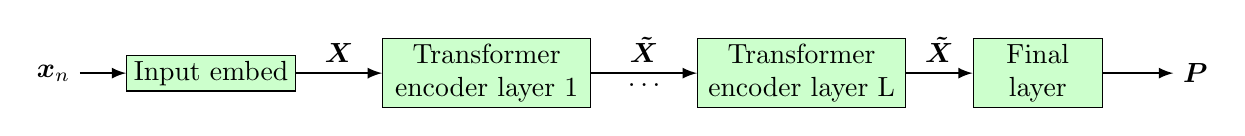
\begin{tikzpicture}
		
		\node (x) {$\bm{x}_n$};
		
		\node (emblayer) [param, right of=x, text centered, text width=2cm, xshift=1cm] {Input embed};
		
		%\node (X) [right of=emblayer, xshift=1cm] {$\bm{X}$};
		
		\node (trlayer1) [param, right of=emblayer, text centered, text width=2.5cm, xshift=2.5cm] {Transformer encoder layer 1};
		
		\node (trlayerN) [param, right of=trlayer1, text centered, text width=2.5cm, xshift=3cm] {Transformer encoder layer L};
		
		\node (finallayer) [param, right of=trlayerN, text centered, text width=1.5cm, xshift=2cm] {Final layer};
		
		\node (out) [right of=finallayer, xshift=1cm] {$\bm{P}$};
		
		\begin{scope}[thick, black, ->, >=latex]
			\draw (x) -- (emblayer);
			\draw (emblayer) -- (trlayer1) node [midway, above] {$\bm{X}$};
			\draw (trlayer1) -- (trlayerN) node [midway, above] {$\bm{\tilde{X}}$} node [midway, below] {$\ldots$};
			\draw (trlayerN) -- (finallayer) node [midway, above] {$\bm{\tilde{X}}$};
			\draw (finallayer) -- (out);
		\end{scope}	
	\end{tikzpicture}
	
\vspace{4em}
As usual, green boxes are functions with trainable parameters

$\bm{\tilde{X}}$ is just a placeholder for \textbf{updated} token embeddings matrix $\bm{X}$	
	\vspace{4em}

	
\end{frame}	







\begin{frame}{BERT (encoding-only transformer, forward pass)}
	
	\vspace{-2em}
	\begin{minipage}[t][10cm][t]{15cm}
		\begin{algorithmic}[1]
			\Function{ETransformer}{$\bm{x} ; \bm{\mathcal{W}}$}
			\State $\ell \gets \text{length}(\bm{x})$
			\State for $t \in [\ell]: \bm{e}_t \gets \bm{W_e}[x[t],:] + \bm{W_p}[t,:]$
			\Comment{Token emb. + positional emb.}
			\State $\bm{X} \gets \text{Stack row-wise}[\bm{e}_1, \bm{e}_2, \ldots \bm{e}_{\ell}]$
			\For{$l = 1, 2, \dots, L$}
			\State $\bm{X} \gets \bm{X} + \textsc{MHAttention}(\bm{X} | \bm{\mathcal{W}}_l)$
			\Comment{Multi-head att., residual conn}
			\State $\bm{X} \gets \textsc{LayerNormPerRow}(\bm{X} | \bm{\gamma^1}_l, \bm{\beta^1}_l)$
			\State $\bm{X} \gets \bm{X} + \left(
			\textsc{GELU}(\bm{X} \bm{W}^\text{mlp1}_l +_{\text{(row)}} \bm{b}^\text{mlp1}_l )
			\bm{W}^{\text{mlp2}}_l +_{\text{(row)}} \bm{b}^{\text{mlp2}}_l \right)$
			\Comment{MLP}
			\State $\bm{X} \gets \textsc{LayerNormPerRow}(\bm{X} | \bm{\gamma^2}_l, \bm{\beta^2}_l)$
			\EndFor
			\State $\bm{X} \gets \textsc{GELU}(\bm{X} \bm{W_f}  +_{\text{(row)}} \bm{b_f} )$
			\State $\bm{X} \gets \textsc{LayerNormPerRow}(\bm{X} | \bm{\gamma}_l, \bm{\beta}_l)$
			\State \Return $\bm{P} = \softmax(\bm{X} \bm{W_u}) $
			\Comment{Project to vocab., probabilities}
			\EndFunction
		\end{algorithmic}
		
	\end{minipage}
\end{frame}




\section{Input and pre-training}

\begin{frame}{BERT: Tokenization}
	
	Tokenizing into a multilingual WordPiece inventory
	
	\begin{itemize}
		\item Recall that WordPiece units are sub-word units
		\item 30,000 WordPiece units (newer models 110k units, 100 languages)
	\end{itemize}
	
	Implications: BERT can "consume" any language
	
	
\end{frame}


\begin{frame}{BERT: Input representation}
	
	\begin{itemize}
		\item Each WordPiece token from the input is represented by a \textbf{WordPiece embedding} (randomly initialized)
		\item Each position from the input is associated with a \textbf{positional embedding} (also randomly initialized)
		\item Input length limited to \textbf{512} WordPiece tokens, using \texttt{<PAD>}ding
		\item Special tokens
		\begin{itemize}
			\item The fist token is always a special token \textbf{[CLS]}
			\item If the task involves two sentences (e.g., NLI), these two sentences are separated by a special token \textbf{[SEP]}; also special two \textbf{segment position embeddings} 
		\end{itemize}
		
	\end{itemize}
	
\end{frame}




\begin{frame}{BERT: Input representation summary}
	
	\begin{figure}
		\includegraphics[width=\linewidth]{img/bert-input.png}	
	\end{figure}
	
\end{frame}



\section{Pre-training}


\begin{frame}{BERT: Self-supervised multi-task pre-training}
	
Prepare two auxiliary tasks that need no labeled data
	
\begin{columns}
% columns tend to stretch over entire slide, add negative to the left
\hspace*{-9em}\begin{column}{0.48\textwidth}
\begin{small}
\noindent Task 1: Cloze-test task
\begin{itemize}
	\item 	Predict the masked WordPiece unit (multi-class, 30k classes)
\end{itemize}


Task 2: Consecutive segment prediction

\begin{itemize}
	\item Did the second text segment appeared after the first segment? (binary)
\end{itemize}
\end{small}
\end{column}
\hspace*{-9.5em}\begin{column}{0.48\textwidth}
\includegraphics[width=\linewidth]{img/bert-pretraining.png}
\end{column}
\end{columns}

\end{frame}




\begin{frame}{BERT: Pre-training data generation}
	
	Take the entire Wikipedia (in 100 languages; 2,5 billion words)
	
	To generate a single training instance, sample two segments (max combined length 512 WordPiece tokens)
	
	\begin{itemize}
		\item For Task 2, replace the second segment randomly in 50\% (negative samples)
		\item For Task 1, choose random 15\% of the tokens, and in 80\% replace with a [MASK] 
	\end{itemize}
	
	
\end{frame}


\begin{frame}{BERT: Pre-training data -- Simplified example}
	
	\begin{columns}
		\begin{column}{0.9\linewidth}
			\begin{figure}
				\includegraphics[width=\linewidth]{img/bert-pretraining2.png}
			\end{figure}
		\end{column}
		\begin{column}{0.5\linewidth}
			\begin{small}
				
				\begin{itemize}
					\item $<$PAD$>$ding is missing
					\item The actual segments are longer and not necessarily sentences (just spans)
					\item The WordPiece tokens match full words here
				\end{itemize}
			\end{small}
		\end{column}
	\end{columns}
	
	
\end{frame}




\begin{frame}{BERT: pre-training by masked language modeling}
	
	\vspace{-2em}	
	\begin{minipage}[t][10cm][t]{15cm}
		\begin{algorithmic}[1]
			\Function{ETraining}{$\left\{ \bm{x}_n \right\}_{n = 1}^{N_\text{data}}$ seqs,  $\bm{\theta}$ init.\ params; $p_{\text{mask}} \in (0, 1)$, $N_\text{epochs}$, $\eta$}
			\For{$i \in [N_{\text{epochs}}]$}
			\For{$n \in [N_{\text{data}}]$}
			\State $\ell \gets \text{length}(\bm{x}_n)$
			\For{$t \in [\ell]$}
			\State $\tilde{\bm{x}}_n[t] \gets \texttt{<mask\_token>}$ with prob.\ $p_{\text{mask}}$, otherwise $\bm{x}_n[t]$
			\EndFor
			\State $\tilde{T} \gets \left\{ t \in [\ell] : \tilde{\bm{x}}_n[t] = \texttt{<mask\_token>} \right\}$
			\Comment{Indices of masked tokens}
			\State $\bm{P_{\theta}} \gets \textsc{ETransformer}(\tilde{\bm{x}}_n | \bm{\theta})$
			\State $\text{loss}_{\bm{\theta}} \gets - \sum_{t \in \tilde{T}} \log \bm{P_{\theta}} [t, \bm{x}_n[t]] $
			\State $\bm{\theta} \gets \bm{\theta} - \eta \cdot \nabla \text{loss}_{\bm{\theta}}$
			\EndFor
			\EndFor
			\State \Return $\bm{\theta}$
			\EndFunction
		\end{algorithmic}
		
	\end{minipage}
\end{frame}




\begin{frame}{Simple example explaining lines 6--7 (masking)}
	$
	\begin{pmatrix}
		\text{The} &
		\text{cat} &
		\text{sat}
	\end{pmatrix}
	\rightarrow
	\bm{x}_n =
	\begin{pmatrix}
		21 &
		11987 &
		5438
	\end{pmatrix}
	\quad \text{(Indices in $V$)}
	$
	
	Random masking (index of \texttt{<mask\_token>} = 50001):
	\begin{enumerate}
		\item For $t = 1$, the random outcome is "mask"
		\item For $t = 2$, the random outcome is "keep"
		\item For $t = 3$, the random outcome is "mask"
	\end{enumerate}
	$
	\bm{\tilde{x}}_n =
	\begin{pmatrix}
		50001 &
		11987 &
		50001
	\end{pmatrix},
	\tilde{T} = \left\{ 1, 3 \right\}
	$
	
	
	
\end{frame}



\begin{frame}{Explaining line 9 (negative log likelihood)}
	
	$
	\begin{pmatrix}
		\text{The} &
		\text{cat} &
		\text{sat}
	\end{pmatrix}
	\rightarrow
	\bm{x}_n =
	\begin{pmatrix}
		21 &
		11987 &
		5438 
	\end{pmatrix},
	\bm{\tilde{x}}_n =
	\begin{pmatrix}
		50001 &
		11987 &
		50001
	\end{pmatrix},
	\tilde{T} = \left\{ 1, 3 \right\}
	$
	
	$\bm{P_{\theta}} \gets \textsc{ETransformer}(\tilde{\bm{x}}_n | \bm{\theta})$
	$$
	\bm{P_{\theta}} =
	\begin{pmatrix}
		0.001 & 0.0007 & \ldots & 0.0003 \\
		0.0013 & 0.0065 & \ldots & 0.0001 \\
		0.079 & 0.015 & \ldots & 0.0001 \\
	\end{pmatrix}
	$$
	
	$\bm{P_{\theta}} \in (0,1)^{\ell_{\text{x}} \times N_{\text{V}}}$, where each row of $\bm{P}$ is a distribution over the vocabulary
	
\end{frame}


\begin{frame}{Explaining line 9 (negative log likelihood), $t = 1$}
	
	\begin{small}
		$\bm{x}_n = (21, 11987, 5438), \bm{\tilde{x}}_n = (50001, 11987, 50001), \tilde{T} = \left\{ 1, 3 \right\}$
		
		$
		\bm{P_{\theta}} =
		\begin{pmatrix}
			0.001 & \ldots & 0.0041_{21} & \ldots 0.0003 \\
			\vdots &  &  &  \\
		\end{pmatrix}
		$
	\end{small}	
	
	For $t = 1$, the model should learn to predict "The" (index 21)
	
	Gold: $\bm{y} = (0, 0, \ldots, 1_{21}, \ldots, 0) \in \mathbb{R}^{N_{\text{V}}}$
	
	Pred: $\bm{\hat{y}} = \bm{P_{\theta}}[1,:] = (0.001, \ldots, 0.0041_{21}, \ldots 0.0003) \in \mathbb{R}^{N_{\text{V}}}$
	
	\begin{block}{Recall: Categorical cross entropy loss}
		$L (\bm{\hat{y}, \bm{y}}) := - \sum_{k = 1}^{K} \bm{y}_{[k]} \log \left(  \bm{\hat{y}}_{[k]} \right)$ \\
		$= - 1 \cdot \log (\bm{\hat{y}}[21])
		= - \log(\bm{P_{\theta}}[1, 21])$ \\
		$= - \log(\bm{P_{\theta}}[1, \bm{x}_n[1]]) 
		= - \log(\bm{P_{\theta}}[t, \bm{x}_n[t]])$	
	\end{block}
	
\end{frame}


\begin{frame}{Explaining line 9 (negative log likelihood), $t = 3$}
	
	\begin{small}
		$\bm{x}_n = (21, 11987, 5438), \bm{\tilde{x}}_n = (50001, 11987, 50001), \tilde{T} = \left\{ 1, 3 \right\}$
		
		$
		\bm{P_{\theta}} =
		\begin{pmatrix}
			\vdots &  \cdots &  \cdots &  \\
		\end{pmatrix}
		$
	\end{small}	
	
	For $t = 3$, the model should learn to predict "sat" (id 5438)
	
	\begin{block}{Categorical cross entropy loss}
		$L (\bm{\hat{y}, \bm{y}}) := - \sum_{k = 1}^{K} \bm{y}_{[k]} \log \left(  \bm{\hat{y}}_{[k]} \right)$ \\
		$= - 1 \cdot \log (\bm{\hat{y}}[5438])
		= - \log(\bm{P_{\theta}}[3, 5438])
		= - \log(\bm{P_{\theta}}[t, \bm{x}_n[t]])$	
	\end{block}
	
	
	Sum over all masked token positions in $\tilde{T}$ gives us line 9:\\
	$$\text{loss}_{\bm{\theta}} \gets - \sum_{t \in \tilde{T}} \log \bm{P_{\theta}} [t, \bm{x}_n[t]] $$
	
\end{frame}







\section{Downstream tasks and fine-tuning}

\begin{frame}{BERT: Representing various NLP tasks}
	
	\begin{figure}
		\includegraphics[width=0.5\linewidth]{img/task1.png}
	\end{figure}


\begin{tikzpicture}[overlay, remember picture] 
	\node at (current page.north east)[ref] {	That explains the special [CLS] token at sequence start \par};
\end{tikzpicture}
	
\end{frame}



\begin{frame}{BERT: Representing various NLP tasks}
	
	\begin{figure}
		\includegraphics[width=0.6\linewidth]{img/task2.png}
	\end{figure}
	
	
\end{frame}



\begin{frame}{BERT: Representing various NLP tasks}
	
	\begin{figure}
		\includegraphics[width=0.5\linewidth]{img/task3.png}
	\end{figure}
	
	
	Not conditioned on surrounding predictions	
	
\end{frame}



\begin{frame}{BERT pre-training time}
		
	Pretraining BERT took originally 4 days on 64 TPUs\footnote{Can be done more efficiently, see, e.g., \citet{izsak-etal-2021-train}}
	
	\bigskip
	
	Once pre-trained, transfer and "fine-tune" on your small-data task and get competitive results


	
\begin{tikzpicture}[overlay, remember picture] 
	\node at (current page.north east)[ref] {\fullcite{izsak-etal-2021-train} \par};
\end{tikzpicture}

	
\end{frame}


\begin{frame}{Recap}
	
	BERT stays on the shoulders of many clever concepts and techniques, mastered into a single model
	
\textbf{What do we know about how BERT works?}

	
\emph{``BERTology has clearly come a long way, but it is fair to say we still have more questions than answers about how BERT works.''} --- \citet{Rogers.et.al.2020.BERT}\footnote{Highly recommended reading!}
	
	
\begin{tikzpicture}[overlay, remember picture] 
	\node at (current page.north east)[ref] {\fullcite{Rogers.et.al.2020.BERT} \par};
\end{tikzpicture}
	
\end{frame}



\section{Sentence BERT}


\begin{frame}{Motivation for Sentence BERT}

BERT --- state-of-the-art performance on sentence-pair tasks (e.g, semantic textual similarity), but

\begin{itemize}
\item both sentences fed into the network $\to$ massive computational overhead
\item ``finding the most similar pair in a collection of 10,000 sentences requires about 50 million inference computations (~65 hours) with BERT"
\end{itemize}

BERT unsuitable for semantic similarity search or unsupervised tasks like clustering

\begin{tikzpicture}[overlay, remember picture] 
	\node at (current page.north east)[ref] {\fullcite{Reimers.Gurevych.2019.EMNLP} \par};
\end{tikzpicture}


\end{frame}



\begin{frame}{Sometimes we need just `suitable' sentence embeddings}

For \textbf{semantic clustering} or \textbf{semantic search} --- we map each sentence to a vector space

\begin{itemize}
\item semantically similar sentences are close to each other
\end{itemize}

How to use BERT for that?

\begin{itemize}
\item average the BERT output layer (known as BERT embeddings)
\item use the first token (the [CLS] token) output
\end{itemize}

$\to$ this practice yields rather bad sentence embeddings, often worse than averaging static word embeddings


\begin{tikzpicture}[overlay, remember picture] 
	\node at (current page.north east)[ref] {\fullcite{Reimers.Gurevych.2019.EMNLP} \par};
\end{tikzpicture}


\end{frame}




\begin{frame}{Fine-tune S-BERT on sentence pair classification}

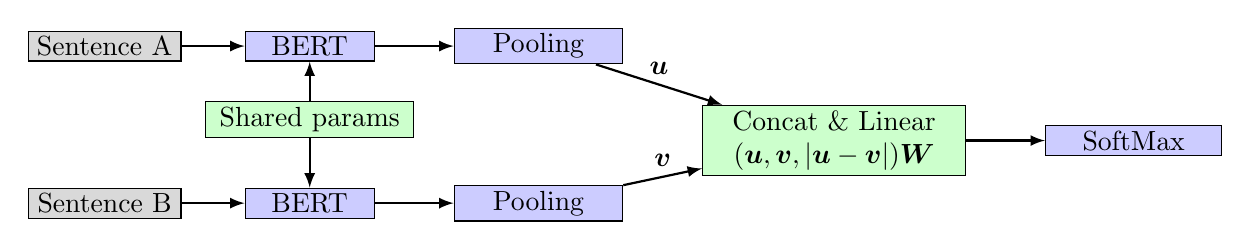
\begin{tikzpicture}

\node (in1) [constant, text centered, text width=1.8cm] {Sentence A};

\node (in2) [constant, text centered, text width=1.8cm, below=1.6 cm of in1] {Sentence B};

\node (bert1) [neuron, right=0.8 cm of in1, text centered, text width=1.5cm] {BERT};

\node (bert2) [neuron, right=0.8 cm of in2, text centered, text width=1.5cm] {BERT};

\node (params) [param, below=0.5 cm of bert1, text centered, text width=2.5cm] {Shared params};

\node (pooling1) [neuron, right=1 cm of bert1, text centered, text width=2cm] {Pooling};

\node (pooling2) [neuron, right=1 cm of bert2, text centered, text width=2cm] {Pooling};

\node (concat) [param, right=1 cm of pooling1, yshift=-1.2cm, text centered, text width=3.2cm] {Concat \& Linear $(\bm{u}, \bm{v}, \abs{\bm{u} - \bm{v}})\bm{W}$};

\node (softmax) [neuron, right=1 cm of concat, text centered, text width=2.1cm] {SoftMax};


\begin{scope}[thick, black, ->, >=latex]
	\draw (in1) -- (bert1);
	\draw (in2) -- (bert2);
	\draw (params) -- (bert1);
	\draw (params) -- (bert2);
	\draw (bert1) -- (pooling1);
	\draw (bert2) -- (pooling2);
	\draw (pooling1) -- (concat) node [midway, above] {$\bm{u}$};
	\draw (pooling2) -- (concat) node [midway, above] {$\bm{v}$};
	\draw (concat) -- (softmax);
%	\draw (trlayer1) -- (trlayerN) node [midway, above] {$\bm{\tilde{X}}$} node [midway, below] {$\ldots$};
%	\draw (trlayerN) -- (finallayer) node [midway, above] {$\bm{\tilde{X}}$};
%	\draw (finallayer) -- (out);
\end{scope}	
\end{tikzpicture}


Training data:
\begin{itemize}
\item SNLI (570,000 sentence pairs)
\item MultiNLI (430,000 sentence pairs)
\end{itemize}




\end{frame}




\begin{frame}{S-BERT provided superior sentence embeddings}

\begin{figure}
\includegraphics[width=\linewidth]{img/sbert-eval.jpg}
\caption{Evaluation of SBERT sentence embeddings using the SentEval toolkit. SentEval evaluates sentence embeddings on different sentence classification tasks by training a logistic regression classifier using the sentence embeddings as features.}
\end{figure}

\begin{tikzpicture}[overlay, remember picture] 
	\node at (current page.north east)[ref] {\fullcite{Reimers.Gurevych.2019.EMNLP} \par};
\end{tikzpicture}


\end{frame}



\begin{frame}{S-BERT efficiency}

``For example, clustering of 10,000 sentences with hierarchical clustering requires with BERT about 65 hours (50 Million sentence combinations). With SBERT, we were able to reduce the effort to about 5 seconds."

Nils' guest lecture (3 parts):
\begin{small}
\begin{itemize}
\item \url{https://www.youtube.com/watch?v=qmN1fJ7Fdmo}
\item \url{https://www.youtube.com/watch?v=0RV-q0--NLs}
\item \url{https://www.youtube.com/watch?v=t4Gf4LruVZ4}
\end{itemize}
\end{small}


\begin{tikzpicture}[overlay, remember picture] 
	\node at (current page.north east)[ref] {\fullcite{Reimers.Gurevych.2019.EMNLP} \par};
\end{tikzpicture}


\end{frame}



\begin{frame}{License and credits}

	\begin{columns}
		\begin{column}{0.7\textwidth}
			Licensed under Creative Commons Attribution-ShareAlike 4.0 International (CC BY-SA 4.0)
		\end{column}
		\begin{column}{0.2\textwidth}
			\includegraphics[width=0.9\linewidth]{img/cc-by-sa-icon.pdf}
		\end{column}
	\end{columns}
	
	\bigskip
	
	Credits
	
	\begin{scriptsize}
		
		Ivan Habernal
		
		Content from ACL Anthology papers licensed under CC-BY \url{https://www.aclweb.org/anthology}
		
	
	\end{scriptsize}
	
\end{frame}





\end{document}

